\chapter{Localization}

In the previous chapters, we have covered the steps to obtain a position of
an object in 2D images. In this chapter, we will take a closer look at
obtaining a position of an object in the world coordinates by combining
information from multiple cameras.

At this point we have computed not only intristic matrices of the cameras but
also the rotation matrix and the translation vector (from the mono camera
calibration and stereo calibration). Our goal is to get a position of the
object in world coordinates from a tuple of coordinates from the images taken by
cameras.

\section{Projection matrices}
Projection matrices provide us a way to transform world coordinates to image
coordinates. The first step is to find out projection matrices for both
cameras, and then we will use them for solving the triangulation problem.

We define a projection matrix as a transformation matrix $P$, such that: $x = P
\dot X$, where $X$ denotes a vector of size 4$\times$1 -- homogenous world coordinates
of the object and $x$ denotes homogenous object coordinates in the image plane
of the camera -- a vector 3$\times$1.

\subsection{World coordinate system}
We define the world coordinate system as orthogonal, with the origin in the
center of projection of the first (usually left) camera. The positive part of
the z-axis is pointing in front of the camera and below the camera is positive
y-axis and to the right is positive x-axis. Layout and the coordinate system is
displayed in the figure \ref{fig:coordinate-system}.

\begin{figure}
\centering
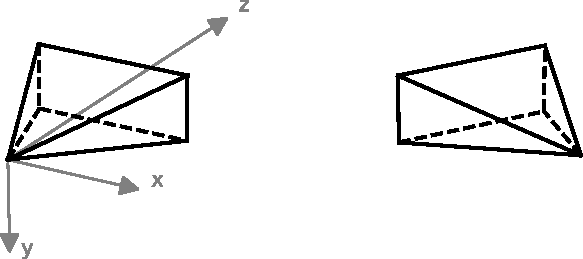
\includegraphics{img/camera-positions}
\caption{Cameras layout and coordinate system}
\label{fig:coordinate-system}
\end{figure}

\subsection{Computing projection matrices}
After defining coordinate systems, we can compute the projection matrices for
both cameras. We use projection matrix decomposition to get the projection matrix
from calibration results.

We decompose projection matrix as $P = K[R|T]$, where $K$ is intristic
camera matrix and $[R|T]$ is extrinsic matrix. $R$ is a rotation matrix and
$T$ is a translation vector. We use this decomposition to compute the projection
matrices.

\emph{First camera}
Since we set the origin of the world coordinate system in the first camera,
the camera has no rotation nor translation to the coordinate system. Therefore
we compute a projection matrix as:

\[
 P_1 = K_1 \cdot \begin{pmatrix}
	I_3 & | & 0_3  
\end{pmatrix}
\]

Where $K_1$ denotes first camera intrinsic parameters matrix, $I_3$ identity
matrix 3$\times$3 and $0_3$ zero vector. Only intristic parameters matrix take
effect on given coordinates, computing from world coordinates in the image plane of the camera.

\emph{Second camera}
For the second camera projection matrix, stereo calibration results will be
used. We know the rotation matrix and translation vector between the cameras,
being able to get coordinates of the second camera relative to the first one.

We now use this information in construction of projection matrix. $P_2 = K_2
\dot [R | T]$, where $K_2$ is second camera intristic parameters matrix, $R$
rotation matrix and $T$ translation vector.

More about the decomposition itself could be found in an article by
\citet{computervisionblog}.

\todo[inline]{V programme aktualne nerobim s distortion coeffs, pretoze uz aj bez toho su rozumne vysledky}

\section{Triangulation}
Now when we know the projection matrices we can formalize our problem as
\begin{equation}
x_1 = P_1X, x_2 = P_2X \label{projection-statements}
\end{equation}
with the goal to find $X$. Since errors may occure during
measurement of $x_1$, $x_2$ and calibration. In further steps we consider that
calibration results are provided with high accurancy compared to measurement of
$x_1$ and $x_2$ (that is the reason to have longer calibration with more images
at once).

\subsection{Simple linear triangulation}
We will now shortly describe how the triangulation is working under the hood.

The results of cross product of vector itself is zero vector. We can write
equation \ref{projection-statements} as crossproduct $x \times (PX) = 0$. We
denote point $x = (x, y, w)$, where $w = 1$ since these coordinates are
homogenous -- in other words up to scale factor $w$.

\todo[inline]{FIX x=(x...)}

We can then rewrite $x \times (PX) = 0$ in the following way:

$$ w(p^{3T}X) - x(p^{2T}X) = 0 $$
$$ y(p^{3T}X) - w(p^{1T}X) = 0 $$
$$ x(p^{2T}X) - y(p^{1T}X) = 0 $$

Where $p^{iT}$ denotes ith row of $P$. Since $w = 1$ we can equally write:

$$ x(p^{3T}X) - (p^{1T}X) = 0 $$
$$ y(p^{3T}X) - (p^{2T}X) = 0 $$
$$ x(p^{2T}X) - y(p^{1T}X) = 0 $$

These equations are linear in the components of X. Only two equations are
linearly independent since the third one could be obtained as the sum $y$
times the first row and $-x$ times the second row.

Therefore an equation of form $AX = 0$ can then be composed using two points $x_1 = (x, y, 1)$ and $x_2 = (m, n, 1)$:

\[
A = \begin{pmatrix}
x(p_1^{3T}X) - (p_1^{1T}X) \\
y(p_1^{3T}X) - (p_1^{2T}X) \\
m(p_2^{3T}X) - (p_2^{1T}X) \\
n(p_2^{3T}X) - (p_2^{2T}X) \\
\end{pmatrix}
\]

For each image two equations were included, giving a total of four equations in
four homogeneous unknowns.

Without an error during measurements a point $X$ satisfying $AX = 0$ would
exist. However, due to the errors it might not exists. As the next step, Homogenous
method (DLT) is used to find the solution. More about the method could be found
in \citet*{multiple-view-geometry}.

\section{Implementation note}
For the triangulation we used OpenCV function triangulatePoints($P_1$, $P_2$,
$x_1$, $x_2$), which is based on simple triangulation method with use of DLT
method for solving equations.
